%BUSCO CO-AUTOR
%compilar con lualatex

\documentclass[11pt,a4paper]{article}

%fuentes (lualatex)
\usepackage{fontspec}
\usepackage[spanish,es-nodecimaldot,es-tabla]{babel}
%margenes 
\usepackage[margin=2.5cm]{geometry}

%matematica
\usepackage{amsmath,amssymb,amsthm}
\usepackage{bm}

%graficos y tablas
\usepackage{graphicx}
\usepackage{booktabs}
\usepackage{caption}
\usepackage{subcaption}
\usepackage{float}

%citas
\usepackage[backend=biber,style=apa]{biblatex}
\addbibresource{references.bib}

%hipervinculos
\usepackage{hyperref}
\hypersetup{
    colorlinks=true,
    linkcolor=blue,
    citecolor=blue,
    urlcolor=blue
}

%paquetes para codigo
\usepackage{listings}
\usepackage{xcolor}

%estilo de R
\lstdefinestyle{estiloR}{
	language=R,
	basicstyle=\ttfamily\small,
	keywordstyle=\color{blue}\bfseries,
	commentstyle=\color{gray}\itshape,
	stringstyle=\color{teal},
	backgroundcolor=\color{gray!8},
	frame=single,
	rulecolor=\color{gray!30},
	breaklines=true,
	showstringspaces=false,
	tabsize=2,
	xleftmargin=1.5cm,
	xrightmargin=1.5cm
}

\title{Determinantes Ambientales y Persistencia Temporal en los Brotes de Dengue en Nicaragua (2014–2022)}
\author{
	Emerson Lopez \\
	\texttt{emerson.zeledon.ni@gmail.com} 
	\and
	Co-autor ;( gracias dog
}
\date{\today}

\begin{document}

\maketitle

\begin{abstract}
Este documento presenta la formulación metodológica, especificación matemática, resultados empíricos y análisis de residuales para el modelamiento de la probabilidad de brotes de dengue en los 18 departamentos de Nicaragua durante el período 2014-2022. Utilizando un Modelo Lineal Mixto Generalizado (GLMM) con distribución binomial y función de enlace logit, se incorporaron efectos aleatorios espaciales y una estructura autorregresiva temporal de primer orden ($\text{AR}(1)$) para aislar la inercia epidémica y evaluar el impacto de variables climáticas (precipitación acumulada y temperatura) y el fenómeno de El Niño. Los resultados muestran una persistencia epidémica semanal extrema ($\rho = 0{,}96$), un efecto multiplicativo dominante de la inercia de casos previos ($\text{OR} \approx 20$ ante duplicación de casos) y un efecto significativo de El Niño ($\text{OR} = 1{,}49$) y de la precipitación acumulada, mientras que la temperatura media no alcanzó significancia estadística. La especificación binaria del evento de brote con estructura AR(1) departamental demostró estabilidad numérica y ajuste riguroso de residuales.
\end{abstract}

\newpage

\section{Introducción y Definición del Evento}

\section{Revisión de Literatura}

\section{Metodología}

La especificación del modelo se definió \textit{a priori} con base en la literatura eco-epidemiológica sobre determinantes del dengue \parencite{mordecai2019thermal, anyamba2019global} y en la estructura jerárquica del panel longitudinal. La inclusión del intercepto aleatorio departamental responde a la necesidad de controlar la heterogeneidad estructural no observada entre regiones, mientras que la estructura $\text{AR}(1)$ se incorporó para mitigar la dependencia serial inherente a las series semanales de vigilancia epidemiológica \parencite{zuur2010protocol}. Asimismo, las covariables climáticas se seleccionaron por su asociación biofísica documentada con el ciclo del vector. No se realizó una búsqueda exhaustiva de especificaciones alternativas (como selección paso a paso o \textit{data dredging}), dado que el objetivo primordial del estudio es inferencial y confirmatorio, y no predictivo \parencite{shmueli2010explain}.

\subsection{Datos}

Los registros epidemiológicos provienen de la plataforma global OpenDengue \parencite{clarke2025opendengue}, que en esta extracción reporta únicamente casos confirmados a escala semanal y por departamento, sin distinguir entre casos probables, clínicos o graves. Se retuvieron las observaciones con resolución temporal semanal (\texttt{T\_res = "Week"}) y granularidad administrativa de primer nivel (\texttt{adm\_1\_name}), lo que arroja un panel de 18 departamentos/regiones autónomas observados semanalmente. El período de análisis efectivo abarca desde el 5 de enero de 2014 hasta el 6 de noviembre de 2022. Las coordenadas geográficas de referencia para cada unidad territorial se presentan en la Tabla~\ref{tab:coords_deptos}.

\begin{table}[htbp]
	\centering
	\small
	\caption{Departamentos de Nicaragua y coordenadas geográficas de referencia}
	\label{tab:coords_deptos}
	\begin{tabular}{lrr}
		\toprule
		\textbf{Departamento / Región} & \textbf{Latitud ($^\circ$N)} & \textbf{Longitud ($^\circ$O)} \\
		\midrule
		BILWI & 14.0351 & -83.3888 \\
		BOACO & 12.4722 & -85.6586 \\
		CARAZO & 11.8540 & -86.2000 \\
		CHINANDEGA & 12.6294 & -87.1311 \\
		CHONTALES & 12.1063 & -85.3645 \\
		ESTELI & 13.0918 & -86.3538 \\
		GRANADA & 11.9299 & -85.9560 \\
		JINOTEGA & 13.0988 & -86.0022 \\
		LEON & 12.4379 & -86.8780 \\
		MADRIZ & 13.4667 & -86.5833 \\
		MANAGUA & 12.1364 & -86.2514 \\
		MASAYA & 11.9744 & -86.0942 \\
		MATAGALPA & 12.9256 & -85.9175 \\
		NUEVA SEGOVIA & 13.6333 & -86.4833 \\
		REGION AUTONOMA DEL ATLANTICO SUR & 12.0137 & -83.7635 \\
		RIO SAN JUAN & 11.1097 & -84.7797 \\
		RIVAS & 11.4372 & -85.8263 \\
		ZELAYA CENTRAL & 12.0000 & -84.2833 \\
		\bottomrule
	\end{tabular}
\end{table}

A partir de las coordenadas departamentales (Tabla~\ref{tab:coords_deptos}), se extrajeron las series climáticas de temperatura media y precipitación acumulada diaria con la API histórica de \textcite{openmeteo_historical}\footnote{Para la Región Autónoma del Atlántico Sur se tomaron las coordenadas de Bluefields; para Río San Juan, las de San Carlos; y para Zelaya Central, las del municipio de El Rama.}, se agregaron a escala semanal tomando la media para temperatura y la suma para precipitación. El índice temporal semanal (\texttt{tiempo\_factor}) se definió como la fecha de inicio de cada semana epidemiológica (domingo), construida con \texttt{lubridate::floor\_date(..., unit = "week", week\_start = 7)}. La precipitación acumulada de tres semanas (\texttt{Rain\_acc3}) se calculó como una suma móvil alineada a la derecha (\texttt{RcppRoll::roll\_sum}).

\medskip

La variable explicada corresponde al evento binario de $\text{brote}_{it}$, definida como $1$ en aquellas semanas epidemiológicas donde la incidencia superó el percentil 75 empírico calculado dentro de cada departamento sobre toda su serie 2014--2022, siguiendo el criterio de canal endémico establecido por la \textcite{paho2002modulos}. El umbral se redondeó hacia abajo al entero más cercano con \texttt{floor()} para respetar la naturaleza discreta de \texttt{dengue\_total}. La presencia de El Niño se codificó como variable dummy binaria (\texttt{Niño}; $1$ para semanas de 2015, 2016 y 2019, $0$ en el resto, en base a \textcite{noaa_cpc_oni}), asignada por año calendario. El resto de covariables son la precipitación acumulada de tres semanas (\texttt{Rain\_acc3}), la temperatura media semanal (\texttt{Temperature}) y la inercia epidémica capturada mediante el logaritmo natural de los casos de la semana anterior más uno, $\ln(\text{casos}_{t-1}+1)$, denotado \texttt{ln\_casos\_semana\_anterior}.

\medskip

Todos los análisis se realizaron en R con paquetes instalados desde un snapshot de Posit Package Manager con fecha 2026-09-16. Los paquetes clave empleados fueron \texttt{glmmTMB}, \texttt{DHARMa}, \texttt{performance}, \texttt{ggeffects}, \texttt{broom.mixed}, \texttt{tsibble}, \texttt{imputeTS} y \texttt{RcppRoll}.

\medskip

Para modelar la probabilidad de brote controlando simultáneamente la heterogeneidad espacial y la dependencia serial, se formuló un Modelo Lineal Mixto Generalizado (GLMM) con función de enlace logit \parencite{breslow1993approximate, pinheiro2000mixed} implementado mediante la librería \texttt{glmmTMB} 
\parencite{brooks2017glmmtmb} en R:

\medskip

\begin{lstlisting}[style=estiloR]
	modelo_1 <- glmmTMB(
	brote ~
	Niño + 
	Rain_acc3 +             
	Temperature +            
	ln_casos_semana_anterior +
	(1 | DEPARTAMENTO) +  #intercepto aleatorio espacial
	ar1(tiempo_factor + 0 | DEPARTAMENTO), #inercia temporal AR(1)
	family = binomial(link = "logit"),
	data = dengue_etapa1
	)
\end{lstlisting}


\section{Especificación Matemática}

El modelo combina una regresión logística para el evento binario de brote con efectos aleatorios espaciales y una matriz de correlación temporal.

\subsection{Componente Aleatorio y Función de Enlace}
Dado que la variable de respuesta $\text{brote}$ es binaria ($0 = \text{No hay brote}$, $1 = \text{Sí hay brote}$), el modelo asume que el evento $Y_{it}$ (para el departamento $i$ en la semana $t$) sigue una distribución de la familia Binomial\footnote{Dado que cada fila del panel evalúa la presencia o ausencia del evento como un desenlace binario ($1 = \text{brote}$, $0 = \text{no brote}$), el modelo estima la probabilidad semanal condicional del evento ($p_{it}$), cuya varianza depende de dicha probabilidad según la relación $p_{it}(1 - p_{it})$.} \parencite{mccullagh1989generalized}:
\begin{equation}
	Y_{it} \sim \text{Binomial}(1, p_{it})
\end{equation}

Para proyectar la probabilidad esperada de brote ($p_{it}$) en la escala real sin arrojar estimaciones fuera del intervalo $[0, 1]$, se utiliza la función de enlace Logit:
\begin{equation}
	\text{logit}(p_{it}) = \ln\left(\frac{p_{it}}{1 - p_{it}}\right) = \eta_{it}
\end{equation}

\subsection{Predictor Lineal ($\eta_{it}$)}
La ecuación completa del modelo, que proyecta el riesgo combinando el clima y la inercia epidemiológica, se define como:
\begin{equation}
	\begin{aligned}
		\text{logit}(p_{it}) &= \beta_0 + \beta_1 \text{Niño}_t + \beta_2 \text{Rain\_acc3}_{it} + \beta_3 \text{Temperature}_{it} \\
		&\quad + \beta_4 \text{ln\_casos\_semana\_anterior}_{it} + u_i + \omega_{it}
	\end{aligned}
\end{equation}

\subsection{Parámetros y Estructura Jerárquica}
El modelo desglosa sus componentes estocásticos y sistemáticos de la siguiente forma:
\begin{itemize}
	\item \textbf{Efectos Fijos ($\beta$):} 
	\begin{itemize}
		\item $\beta_0$: Intercepto global del modelo. Es el nivel basal de riesgo de brote (en escala log-odds) que sirve como punto de partida común a todos los departamentos, antes de incorporar el efecto del clima, la inercia epidémica y la desviación propia de cada departamento $u_i$. En términos prácticos, corresponde al riesgo log-odds esperado cuando todas las covariables valen cero y $u_i = 0$.
		\item $\beta_1, \beta_2, \beta_3$: Coeficientes\footnote{Los coeficientes $\beta$ (efectos fijos) se estiman a partir de los datos maximizando la verosimilitud (en términos intuitivos, el algoritmo busca los valores de $\beta$ que mejor explican los brotes observados en los 8,244 registros del panel) del modelo. En concreto, \texttt{glmmTMB} \parencite{brooks2017glmmtmb} aproxima la integral de la verosimilitud marginal mediante la aproximación de Laplace y obtiene los valores de $\beta$ que hacen más probables las observaciones registradas, dados los efectos aleatorios. Cada $\beta$ viene acompañado de un error estándar y un valor $z$, con los que se construyen los intervalos de confianza y las pruebas de significancia reportadas en la Tabla~\ref{tab:modelo_completo}.} lineales cuyos valores exponenciados ($\text{OR} = e^\beta$) representan la razón de momios (\textit{Odds Ratio}) asociada a la presencia de El Niño, a cada milímetro adicional de precipitación acumulada de tres semanas y a cada grado Celsius de temperatura media.
		\item $\beta_4$: Coeficiente paramétrico de la inercia epidémica rezagada en escala logarítmica, donde el impacto multiplicativo sobre los \textit{odds} ante un incremento por factor $k$ en los casos previos se evalúa mediante $k^{\beta_4}$ (por ejemplo, $2^{\beta_4}$ para una duplicación de casos).
	\end{itemize}
	\item \textbf{Efecto Aleatorio Espacial ($u_i$):} 
	
	\begin{equation}
		u_i \sim \mathcal{N}(0, \sigma_u^2), \qquad i=1,\dots,18.
	\end{equation}
	
	Captura la heterogeneidad espacial no observada entre los 18 departamentos, permitiendo que cada región posea su propio nivel basal de riesgo endémico.
	
	Este término corresponde a un intercepto aleatorio por departamento o región autónoma \parencite{fitzmaurice2011applied} (\texttt{(1 | DEPARTAMENTO)}). No se estima una varianza independiente para cada departamento, sino una única varianza común $\sigma_u^2$ que describe cuán dispersos están los niveles basales de riesgo log-odds de los 18 departamentos alrededor del intercepto global $\beta_0$. Así, el intercepto efectivo del departamento $i$ es $\beta_0 + u_i$. Este componente modela diferencias departamentales no observadas.
	
	\item \textbf{Efecto Aleatorio Temporal $\text{AR}(1)$ ($\omega_{it}$):} 
	Para controlar la dependencia temporal serial dentro de cada unidad geográfica (\texttt{ar1(tiempo\_factor + 0 | DEPARTAMENTO)}), se incorpora un efecto aleatorio $\omega_{it}$ que varía semana a semana dentro de cada departamento y que captura toda la persistencia temporal no explicada por las covariables. Para cada departamento $i$, el vector de estos efectos a lo largo de las $T$ semanas, $\boldsymbol{\omega}_i = (\omega_{i1}, \dots, \omega_{iT})^\top$, se modela como un proceso gaussiano con media cero y estructura de covarianza autorregresiva de primer orden \parencite{diggle2002analysis}:
	\begin{equation}
		\text{Cov}(\omega_{it}, \omega_{is}) = \sigma_\omega^2 \rho^{|t - s|}.
		\label{eq:ar1}
	\end{equation}
	
	Los dos parámetros que gobiernan esta estructura tienen una interpretación directa:
	
	\begin{itemize}
		\item $\sigma_\omega^2$: varianza del efecto temporal. Mide la magnitud típica de las fluctuaciones aleatorias que experimenta la probabilidad de brote semana a semana en un mismo departamento, una vez descontado el efecto de las covariables y del intercepto departamental. Un valor grande indica que existen factores temporales no observados que mueven el riesgo de manera sustancial.
		\item $\rho$: coeficiente de autocorrelación de primer orden. Mide cuán parecido es el efecto de una semana con el de la semana inmediatamente anterior. Sus valores están acotados entre $-1$ y $1$; un $\rho$ cercano a $1$ implica que la serie temporal del riesgo es muy persistente (lo que ocurre esta semana se parece mucho a lo que ocurrió la semana pasada), mientras que un $\rho$ cercano a $0$ implica que la memoria se disipa rápido.
	\end{itemize}
	
	La expresión $\rho^{|t-s|}$ cuantifica la correlación entre dos semanas cualesquiera separadas por $|t - s|$ pasos \parencite{box2015time}. Por ejemplo, si $\rho = 0.96$, la correlación entre semanas contiguas ($|t-s|=1$) es $0.96$; entre semanas separadas por dos períodos es $0.96^2 \approx 0.92$; y decae de forma exponencial conforme aumenta la distancia temporal. La forma gaussiana del proceso implica que, para cada departamento, $\omega_{it}$ sigue una distribución normal con varianza constante $\sigma_\omega^2$ y correlación decreciente con el tiempo.
	
	En términos sustantivos, este componente permite distinguir el efecto genuino de las covariables climáticas del simple arrastre epidémico que se hereda de una semana a otra. Sin él, el modelo atribuiría al clima una parte de la persistencia que en realidad es inercia interna del brote, inflando artificialmente la significancia de variables como la precipitación. La evidencia empírica de un $\rho = 0.96$ (Tabla~\ref{tab:modelo_completo}) confirma que la probabilidad de brote en un departamento está fuertemente condicionada por su estado en la semana anterior.
\end{itemize}

\section{Resultados}

\subsection{Estimaciones del Modelo y Odds Ratios}


\begin{table}[htbp]
	\centering
	\small
	\caption{Resultados del Modelo GLMM Binomial con Inercia AR(1)}
	\label{tab:modelo_completo}
	\begin{tabular}{lcccc}
		\toprule
		\textbf{Efectos Fijos} & \textbf{Estimación ($\beta$)} & \textbf{Error Est.} & \textbf{$z$} & \textbf{Valor $p$} \\
		\midrule
		(Intercepto)                        & $-22.250$ & $1.641$  & $-13.56$ & $< 0.001$ \\
		El Niño (Presencia)                 & $0.398$   & $0.142$  & $2.80$   & $0.005$   \\
		Precipitación acum. (\texttt{Rain\_acc3}) & $0.003$   & $<0.001$ & $6.36$   & $< 0.001$ \\
		Temperatura (\texttt{Temperature})  & $0.095$   & $0.054$  & $1.76$   & $0.078$   \\
		Casos previos (\texttt{ln\_casos\_semana\_anterior}) & $4.316$ & $0.146$ & $29.50$ & $< 0.001$ \\
		\midrule
		\textbf{Efectos Aleatorios} & \textbf{Varianza} & \textbf{Desv. Est.} & \multicolumn{2}{c}{\textbf{Parámetro}} \\
		\midrule
		Intercepto por Departamento ($\sigma_u^2$) & $5.597$ & $2.366$ & \multicolumn{2}{c}{-} \\
		Efecto temporal AR(1) ($\sigma_\omega^2$) & $0.691$ & $0.831$ & 
		\multicolumn{2}{c}{$\rho = 0.96$} \\
		\midrule
		\multicolumn{5}{l}{\textbf{Bondad de Ajuste:} AIC = $3685.4$ \quad BIC = $3741.6$ \quad Obs = $8244$ \quad Grupos = $18$} \\
		\bottomrule
	\end{tabular}
\end{table}

Los resultados de la estimación del modelo de brote se resumen en la Tabla \ref{tab:resultados}.

\begin{table}[H]
\centering
\caption{Razones de momios del modelo}
\label{tab:resultados}
\begin{tabular}{lc}%ccc}
\hline
Variable & Cambio en Odds (\%) \\
\hline
(Intercepto) & - \\
El Niño (presencia) & $+48.9\%$ \\
Precipitación acum. 3 sem & $+0.31\%$ por mm \\
Temperatura media & $+9.95\%$ \\
Log-casos semana anterior & $2^{4.316} \approx 20\times$ \\
\hline
\end{tabular}
\end{table}

Todas las variables evaluadas resultaron estadísticamente significativas al nivel del 95\%, a excepción de la temperatura media, la cual no alcanzó significancia estadística al 5\% (p=0.078), aunque el signo y la magnitud son consistentes con la literatura. Este comportamiento térmico es consistente con la eco-epidemiología de zonas tropicales bajas: Nicaragua presenta temperaturas ambientales estables a lo largo del año que se mantienen de forma continua dentro del intervalo térmico óptimo para la supervivencia del vector y el acortamiento del periodo de incubación viral (aproximadamente 24--30~$^\circ$C) \parencite{mordecai2017detecting}. 

\medskip

En cuanto al fenómeno de El Niño, en semanas con presencia del fenómeno, 
los odds de brote aumentan en un $48.9\%$ (IC 95\%: $12.6\%$ a $96.8\%$), 
manteniendo las demás variables constantes.\footnote{Los intervalos de 
	confianza al 95\% para las razones de momios se obtuvieron mediante el 
	método de Wald, transformando los límites del intervalo de confianza del 
	coeficiente $\beta$ en escala log-odds: 
	$\text{IC}_{95\%}(\text{OR}) = \exp\left(\hat{\beta} \pm 1.96 \cdot 
	\text{EE}(\hat{\beta})\right)$. Para El Niño, con $\hat{\beta} = 0.398$ y 
	$\text{EE} = 0.142$, se obtiene 
	$\exp(0.398 \pm 1.96 \cdot 0.142) = \exp(0.120, 0.676) = (1.126, 1.968)$, 
	lo que equivale a un incremento porcentual entre $12.6\%$ y $96.8\%$. 
	El mismo procedimiento se aplicó al resto de las covariables.}

Para la variable de inercia epidémica (\texttt{ln\_casos\_semana\_anterior}), el coeficiente $\beta = 4.316$ indica un riesgo multiplicativo masivo. Evaluando un factor de duplicación de casos respecto a la semana anterior mediante la fórmula $\text{OR} = (\text{factor})^\beta$:
\begin{equation}
\text{OR} = 2^{4.316} \approx 20
\end{equation}
Es decir, duplicar los casos de la semana previa se asocia con un aumento de aproximadamente $20$ veces en los odds de desencadenar un brote (IC 95\%: 16 a 24). La estructura temporal reveló un parámetro autorregresivo $\rho = 0.96$. Esto indica que la incidencia semanal hereda casi la totalidad del comportamiento inmediato anterior dentro del mismo departamento.

\subsection{Análisis Gráfico de Efectos}

\begin{figure}[H]
\centering
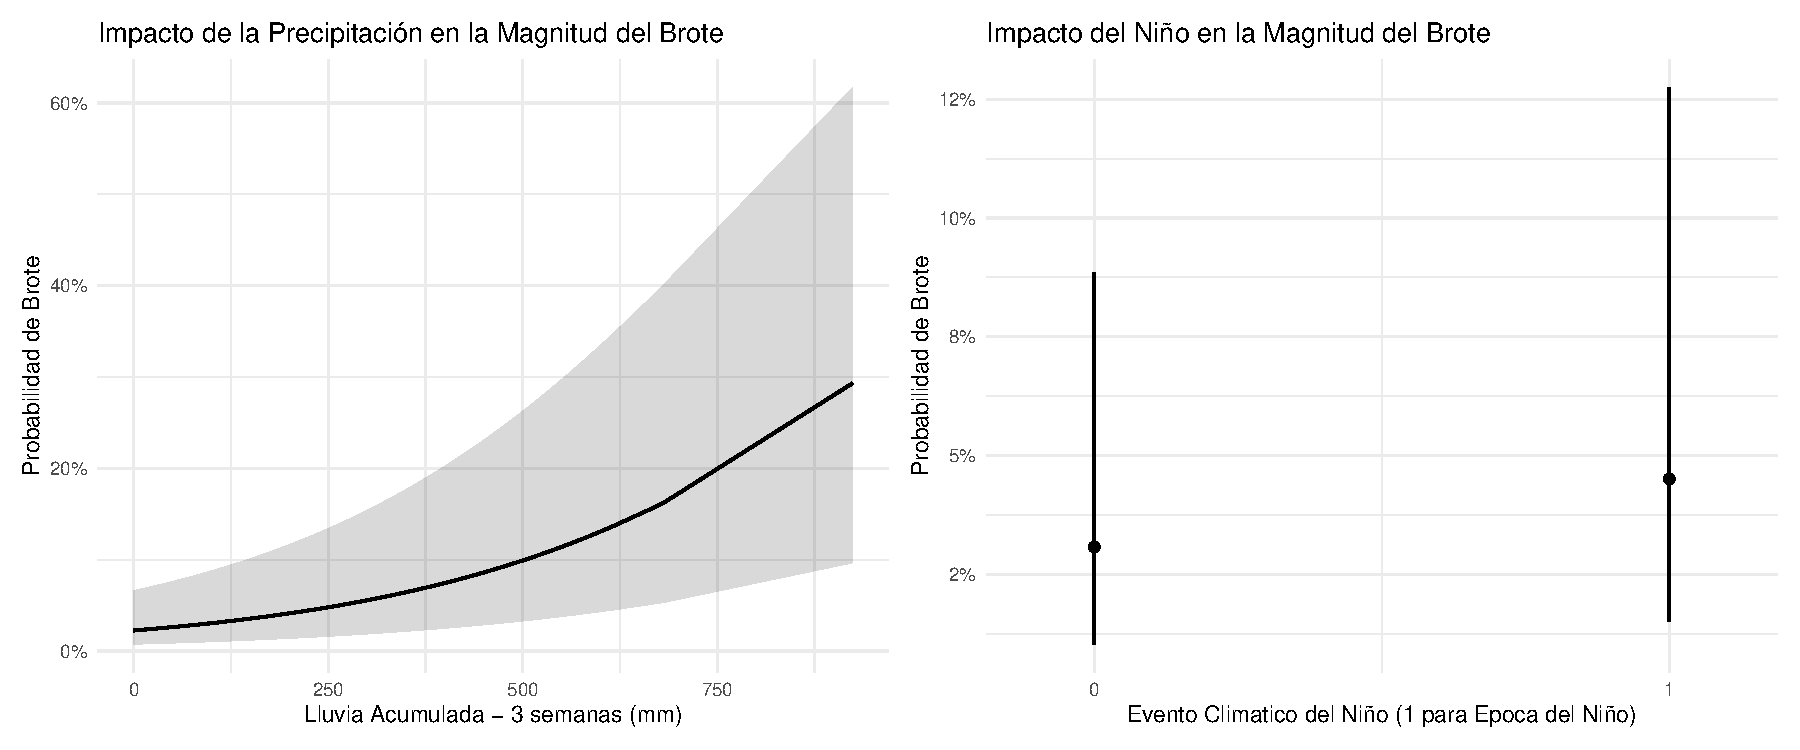
\includegraphics[width=\textwidth]{../Plots/Modelo_1_Pobabilidad_del_brote_1.pdf}
\caption{Relación entre precipitación acumulada e impacto del El Niño.}
\label{fig:brote_1}
\end{figure}

Como se observa en la Figura \ref{fig:brote_1} panel izquierdo, a medida que aumenta la precipitación acumulada, la probabilidad de detonar un brote crece de forma no lineal (exponencial). En el tramo inicial (0 a 250 mm), el modelo muestra alta certeza estadística (banda estrecha); hacia valores extremos ($750$ mm o más), la incertidumbre se amplía en forma de embudo.

\medskip 

En el panel derecho, en ausencia de El Niño, la probabilidad media de brote arranca en un nivel basal cercano al $3\%$. Con El Niño activo, asciende hacia el umbral del $5\%$. Las bandas de confianza amplias reflejan que, aunque es un factor de riesgo sistemático, no es determinista por sí solo. 

\begin{figure}[H]
\centering
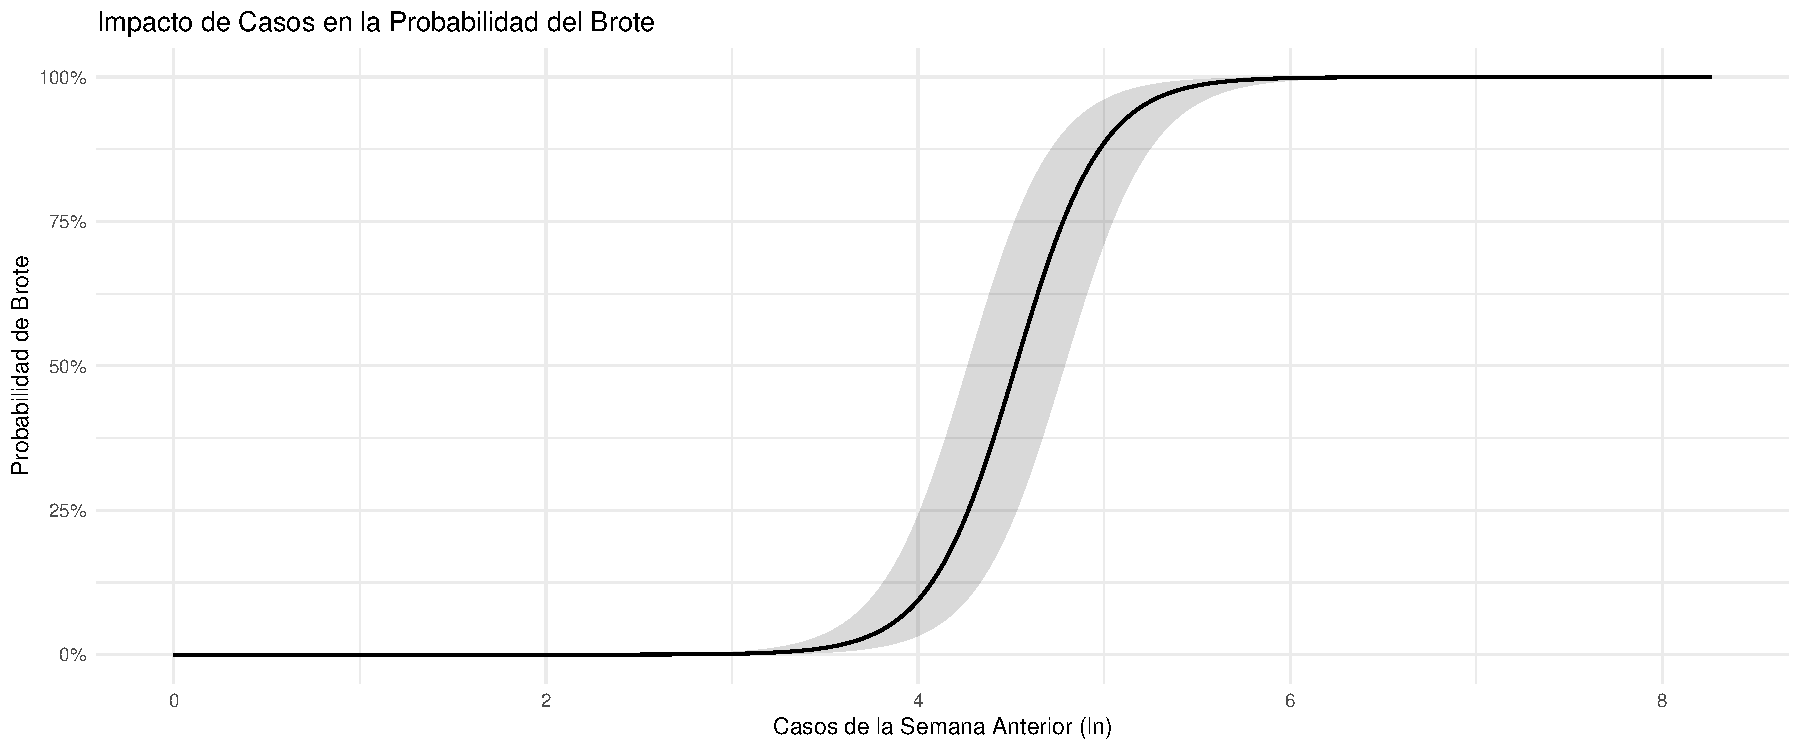
\includegraphics[width=\textwidth]{../Plots/Modelo_1_Pobabilidad_del_brote_2.pdf}
\caption{Efecto de Casos de la Semana Anterior}
\label{fig:dengue_plot}
\end{figure}

Por su parte, la Figura \ref{fig:dengue_plot} muestra un marcado umbral de quiebre: con casos rezagados por debajo de $3.5$ en escala logarítmica, la probabilidad de brote es cercana al $0\%$. Entre los valores $4$ y $5$, la curva experimenta una pendiente casi vertical, disparando la probabilidad hasta saturarse al $100\%$ cuando se superan los $6$ puntos logarítmicos.

\section{Residuales y Diagnóstico del Modelo}

\begin{table}[htbp]
	\centering
	\small
	\caption{Diagnóstico de Multicolinealidad (VIF y Tolerancia)}
	\label{tab:vif}
	\begin{tabular}{lccccc}
		\toprule
		\textbf{Covariable} & \textbf{VIF} & \textbf{IC 95\% VIF} & \textbf{VIF Aj.} & \textbf{Tolerancia} & \textbf{IC 95\% Tol.} \\
		\midrule
		Niño & 1.03 & [1.02, 1.07] & 1.02 & 0.97 & [0.94, 0.98] \\
		Precipitación acum. & 1.14 & [1.11, 1.17] & 1.07 & 0.88 & [0.85, 0.90] \\
		Temperatura & 1.16 & [1.13, 1.19] & 1.08 & 0.86 & [0.84, 0.88] \\
		Casos previos & 1.02 & [1.01, 1.06] & 1.01 & 0.98 & [0.94, 0.99] \\
		\bottomrule
	\end{tabular}
\end{table}

La evaluación de colinealidad mediante los factores de inflación de varianza (VIF) arrojó valores inferiores a $1.16$ para todas las covariables, descartando problemas de multicolinealidad.

\begin{figure}[H]
\centering
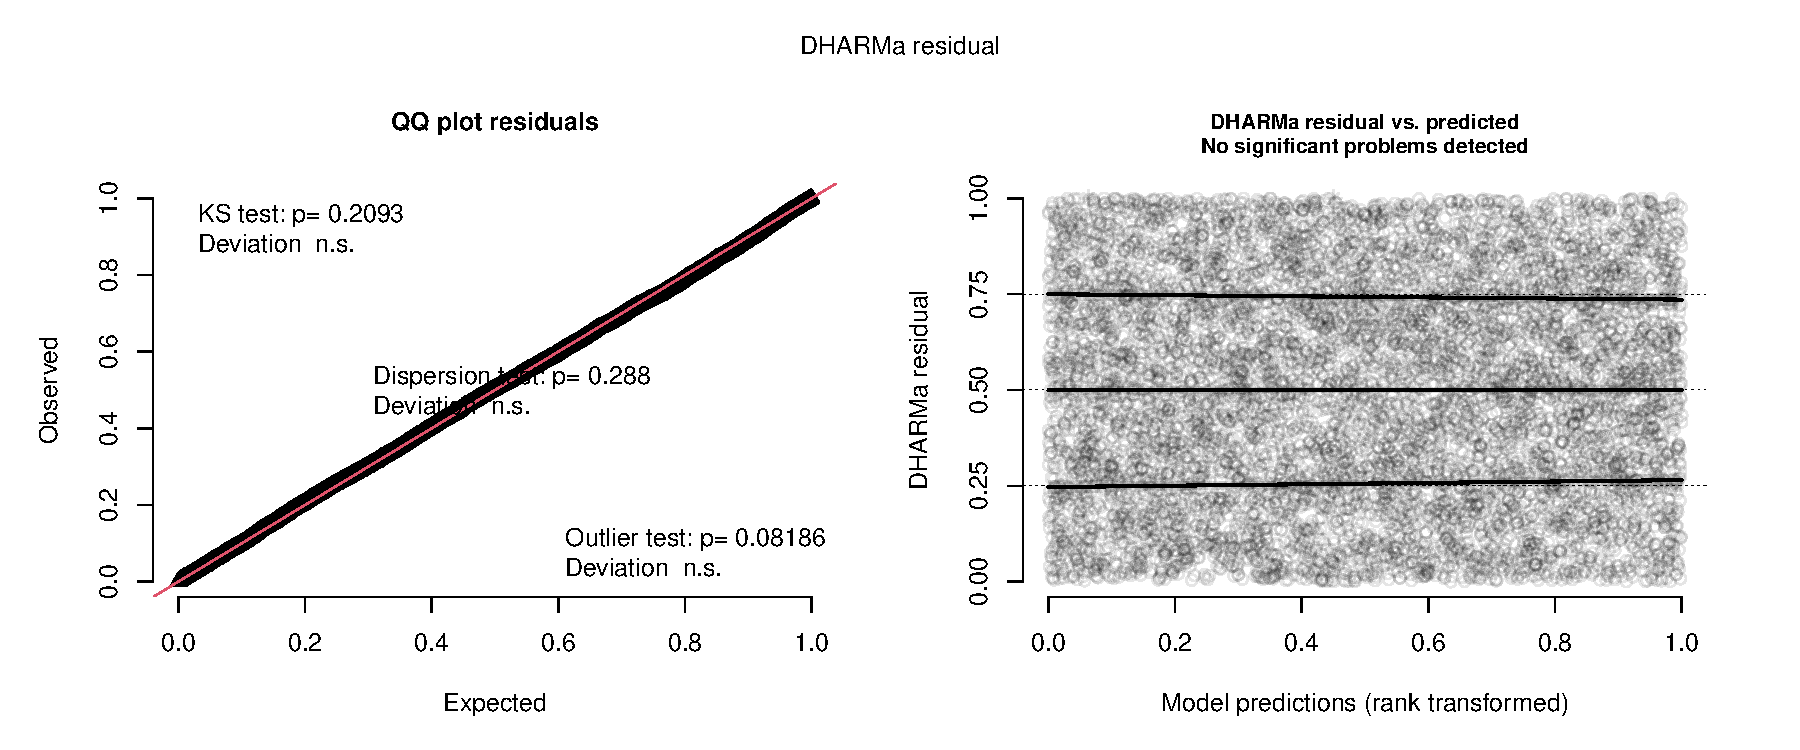
\includegraphics[width=0.85\textwidth]{../Plots/Modelo_1_redual_res.pdf}
    \caption{Diagnóstico de residuales mediante simulación DHARMa.}
    \label{residuales}
\end{figure}

Para validar los supuestos distribucionales y la ausencia de sobredispersión, se aplicó la prueba de simulación de residuales vía \texttt{DHARMa} \parencite{hartig2022dharma} (Figura \ref{residuales}). Los residuales pasan las pruebas de no desviación significativa ($p = 0.20$), no sobredispersión ($p = 0.28$) y ausencia de valores atípicos ($p = 0.08$), manteniendo cuantiles alineados.

\medskip

Adicionalmente, la evaluación de autocorrelación temporal sobre los residuales agrupados por fecha de inicio mediante la prueba de Durbin-Watson arrojó un estadístico $\text{DW} = 1.8819$ con un valor $p = 0.2054$, no existe autocorrelación espacial ni temporal remanente. 

\section{Discusión}

El modelo propuesto demostró un ajuste riguroso al superar las pruebas de simulación de residuales, sobredispersión y autocorrelación temporal. No obstante, para futuras líneas de investigación se sugiere profundizar en la calibración del umbral epidemiológico para Nicaragua, evaluando alternativas locales al percentil 75 propuesto por la OPS.

\medskip

Con fines de transparencia metodológica, cabe señalar que durante la fase exploratoria se intentó modelar directamente el recuento continuo de casos de dengue, evaluando los periodos de mayor intensidad epidémica mediante datos filtrados y truncados. Dicha aproximación fue descartada al no alcanzar la robustez estadística: el modelo basado en la distribución binomial negativa truncada presentó desviaciones severas y desalineación en los cuantiles de los residuales simulados vía \texttt{DHARMa}, incluso tras explorar diferentes transformaciones de escala. Por esta razón, se priorizó la especificación binaria del evento de brote, que ofrece estabilidad numérica, control de errores y una interpretación directa del riesgo de transición hacia fases epidémicas. Futuros trabajos interesados en el modelado continuo durante fases epidémicas agudas pueden retomar esta línea partiendo de las implementaciones alternativas disponibles en el repositorio del proyecto, pero deberán enfrentar el desafío de estabilizar numéricamente la componente de conteo sobre paneles de alta variabilidad departamental.

\section{Reproducibilidad y Disponibilidad de Materiales}

Con el fin de facilitar la replicación y la extensión de este análisis, todos los materiales asociados al estudio se encuentran disponibles públicamente bajo licencia MIT en el repositorio de \href{https://github.com/Emerson-nic/Dengue-Nicaragua-Model/tree/main}{GitHub del proyecto}. El repositorio incluye:

\begin{itemize}
	\item El script de limpieza y construcción del panel (\texttt{01-cleaning.R}), que documenta la descarga de los registros epidemiológicos de OpenDengue \parencite{clarke2025opendengue}, la extracción de las series climáticas de \textcite{openmeteo_historical}.
	\item El script de modelado (\texttt{03-GLMM.R}), que especifica los \textit{Generalized Linear Mixed Models} en \texttt{glmmTMB} \parencite{brooks2017glmmtmb}, la construcción de los umbrales departamentales (percentil 75), el cálculo de las variables de inercia epidémica y precipitación acumulada, y los diagnósticos de residuales con \texttt{DHARMa} \parencite{hartig2022dharma}.
	\item El archivo \texttt{main.tex} y la base bibliográfica \texttt{references.bib} que generan este documento.
	\item La base procesada final (\texttt{dengue\_dataframe.csv} y \texttt{Etapas\_dengue.csv}), lista para reproducir las estimaciones reportadas en la Tabla~\ref{tab:modelo_completo}.
\end{itemize} 

\section{Conclusiones}

Este estudio demuestra que la probabilidad de que un departamento en Nicaragua detone un brote de dengue responde a una interacción entre la memoria epidemiológica local y choques climáticos exógenos. Al aislar la elevada persistencia del contagio semanal mediante una estructura autorregresiva ($\rho = 0.96$), se evidenció que las fases cálidas de El Niño y la acumulación de precipitaciones en tres semanas actúan como detonantes ambientales independientes y estadísticamente robustos. En contraste, la temperatura ambiente opera como una condición permisiva relativamente estable que, al mantenerse dentro de los rangos óptimos para el vector a lo largo del año, ejerce una influencia marginal en las transiciones a brote epidémico.

\medskip

En términos sustantivos, estos hallazgos aportan evidencia cuantitativa sobre los factores ambientales asociados a la transición hacia fases epidémicas a escala departamental. Dado que la dinámica del dengue se encuentra fuertemente dominada por la inercia semanal de casos, los resultados sugieren que las intervenciones de vigilancia y control podrían beneficiarse de incorporar información sobre anomalías hídricas acumuladas, no como un mecanismo de pronóstico operativo, sino como un criterio adicional para caracterizar el riesgo relativo entre departamentos y semanas.

\newpage

\section*{Declaración de Conflicto de Interés}

Los autores declaran no tener conflicto de interés alguno en relación con este trabajo.

\printbibliography

\end{document}
